% IEEE PES General Meeting - Conference Paper Template (IEEEtran)
% Target: 5 pages max incl. figs/refs. Compile with pdfLaTeX.
% Upload this .tex + demo.png to Overleaf (Menu -> Compiler: pdfLaTeX, TeX Live 2024+),
% document class IEEEtran is preinstalled. Final submission must pass IEEE PDF eXpress.
\documentclass[conference, letterpaper, 10pt]{IEEEtran}
\usepackage{graphicx}
\usepackage{amsmath, amssymb}
\usepackage{booktabs}
\usepackage{url}
\usepackage{cite}
\graphicspath{{./}{../results/}{./figs/}}

\title{Grid-Interactive HVAC Load Forecasting and Supervisory Control for Peak Reduction in Hot-Humid Commercial Buildings}

\author{\IEEEauthorblockN{Md. Sabbir Hossain}
\IEEEauthorblockA{Independent Researcher, Dhaka, Bangladesh\\
Shuvo.Hossain101@gmail.com}}

\begin{document}
\maketitle

\begin{abstract}
Commercial HVAC drives 40--60\% of building electricity and a disproportionate share of distribution peaks in hot-humid grids. We present a grid-interactive, physics-informed pipeline coupling ASHRAE psychrometrics and a 2R2C zone model with a gradient-boosting hourly cooling-load forecaster and supervisory control (supply-air-temperature reset, minimum-chiller sequencing, look-ahead pre-cooling). On a 2000~m$^2$ office synthetic dataset (8760~h, Dhaka-like climate, 42.2~kW mean), forecasting reaches MAE 1.55~kW, RMSE 2.76~kW, $R^2$ 0.9907, CVRMSE 8.30\%, NMBE 2.29\% (60-day test), satisfying ASHRAE Guideline~14 hourly limits (30\%/10\%). SAT reset cuts HVAC energy 11.11\% (13.97\% annual) with weekly peak shaving; optimal sequencing saves 24.49\% versus all-chillers-on. The 168-h lag dominates importance (45.8\%), enabling day-ahead flexible-load bidding. The 7-module package runs in under one minute without GPU; 5/5 tests pass.
\end{abstract}

\begin{IEEEkeywords}
Building energy management, HVAC, load forecasting, demand response, peak reduction, chiller sequencing, ASHRAE Guideline 14.
\end{IEEEkeywords}

\section{Introduction}
Electrified cooling is the fastest-growing end use on many South Asian feeders. In Dhaka, commercial HVAC sets distribution peaks, stresses transformers, and inflates demand charges. Grid-interactive efficient buildings (GEBs) that forecast and reshape load are a PES General Meeting priority under \textit{Powering the Digital Era}. Gaps: (i) no trustworthy day-ahead forecasts at meter/plant resolution; (ii) fixed supply-air temperature (SAT) and naive staging waste part-load efficiency and offer no flexibility product. We ask: (Q1) can lightweight ML clear calibration grade? (Q2) what energy \textit{and} peak reductions follow? (Q3) which signals make load dispatchable? Contributions: a forecaster with flexibility outputs, a part-load-consistent energy+peak comparison, and open code mapping building kW to feeder demand-response (DR) potential.

\section{Grid Context and Related Work}
PES treats buildings as distributed energy resources (GEBs, DR, virtual power plants). Guideline~36 sequences and Braun supervisory optima are the controls baseline; boosted trees are Pareto-optimal hourly forecasters; Guideline~14 governs calibration. Unlike pure-ML work, we retain a 2R2C model so pre-cooling has a thermal battery to dispatch, with shifted kWh, shed kW, and rebound characterized for settlements.

\section{Methodology}
\subsection{Electrical-Thermal Interface}
Power is $P = Q_{\mathrm{cool}}/\mathrm{COP} + P_{\mathrm{fan}}$. Psychrometrics (Tetens $p_{\mathrm{sat}}$, $W$, $h$, Magnus dew-point, coil $Q$) give the latent/sensible split; 2R2C gives $Q_{\mathrm{hvac}}$ dynamics with $R$ 1.5/2.5~K/kW, $C$ 2/8~kWh/K. Chiller $\mathrm{COP} = \mathrm{rated}\times f(\mathrm{PLR})\times f(T_{\mathrm{out}})$, $f(\mathrm{PLR})=0.45+0.85\mathrm{PLR}-0.30\mathrm{PLR}^2$. Plant: $2\times175$~kW. Each step yields kW, COP, zone $T$ plus a flexibility band.

\subsection{Data}
Hourly synthetic BMS trends (seed 42), 8760~h at 42.2~kW mean, columns compatible with AMI/BMS exports for field replay.

\subsection{Day-Ahead Forecaster}
Calendar-cyclical plus lag 1/24/168-h features; gradient boosting default; 80/20 chronological split; TimeSeriesSplit CV; MAE/RMSE/CVRMSE/NMBE/$R^2$.

\subsection{Controllers}
Baseline: SAT 13$^\circ$C, all chillers on, constant-volume fan. Reset: 12--16$^\circ$C by outdoor temperature, VAV fan, +2\% COP. Sequencing: fewest chillers above 15\% PLR. MPC proxy: 60\% pre-cool when 32$^\circ$C enters the 4-h horizon inside 22--25.5$^\circ$C. All share one part-load curve so only staging/reset effects are measured.

\section{Case Study Setup}
Laptop, Python~3.11, scikit-learn~1.9; \texttt{examples/run\_demo.py} (60~d); train/evaluate scripts (full year); pytest (5 tests); under 1~min, no GPU. Outputs: \texttt{metrics.json}, \texttt{demo.png}.

\section{Results}
\subsection{Forecasting (Q1)}
60-day: MAE 1.55, RMSE 2.76~kW, CVRMSE 8.30\%, NMBE +2.29\%, $R^2$ 0.9907---PASS. Annual: 1.71, 2.95~kW, 9.82\%, $-1.57\%$, 0.9877---PASS. Importances: lag-168 45.8\%, internal 18.4\%, occupied 17.9\%, $T_{\mathrm{out}}$ 8.1\%.

\begin{table}[htbp]
\caption{Forecast vs.\ ASHRAE Guideline 14 hourly (30\%/10\%).}
\label{tab:forecast}
\centering
\begin{tabular}{lccccc}
\toprule
Split & MAE & RMSE & CVRMSE & NMBE/$R^2$ & G14 \\
\midrule
60-day & 1.55 kW & 2.76 kW & 8.30\% & +2.29\%/0.9907 & PASS \\
Annual & 1.71 kW & 2.95 kW & 9.82\% & $-1.57\%$/0.9877 & PASS \\
\bottomrule
\end{tabular}
\end{table}

\subsection{Energy and Peak (Q2)}
\begin{table}[htbp]
\caption{Energy and savings; weekly peak shaved $\sim$10--12\% under reset.}
\label{tab:energy}
\centering
\begin{tabular}{lcccc}
\toprule
Strategy & 60-d kWh & Save & Year kWh & Save \\
\midrule
Baseline & 4291.1 & --- & 191582.8 & --- \\
SAT reset & 3814.5 & 11.11\% & 164825.4 & 13.97\% \\
Sequencing & --- & --- & 144655.4 & 24.49\% \\
\bottomrule
\end{tabular}
\end{table}

At 42~kW mean, 11--14\% is 4.6--5.9~kW average flexibility per building; 100 buildings aggregate to $\sim$0.5~MW of DR. Pre-cooling shifts $\sim$20~kWh/day off the afternoon peak.

\begin{figure}[htbp]
\centering
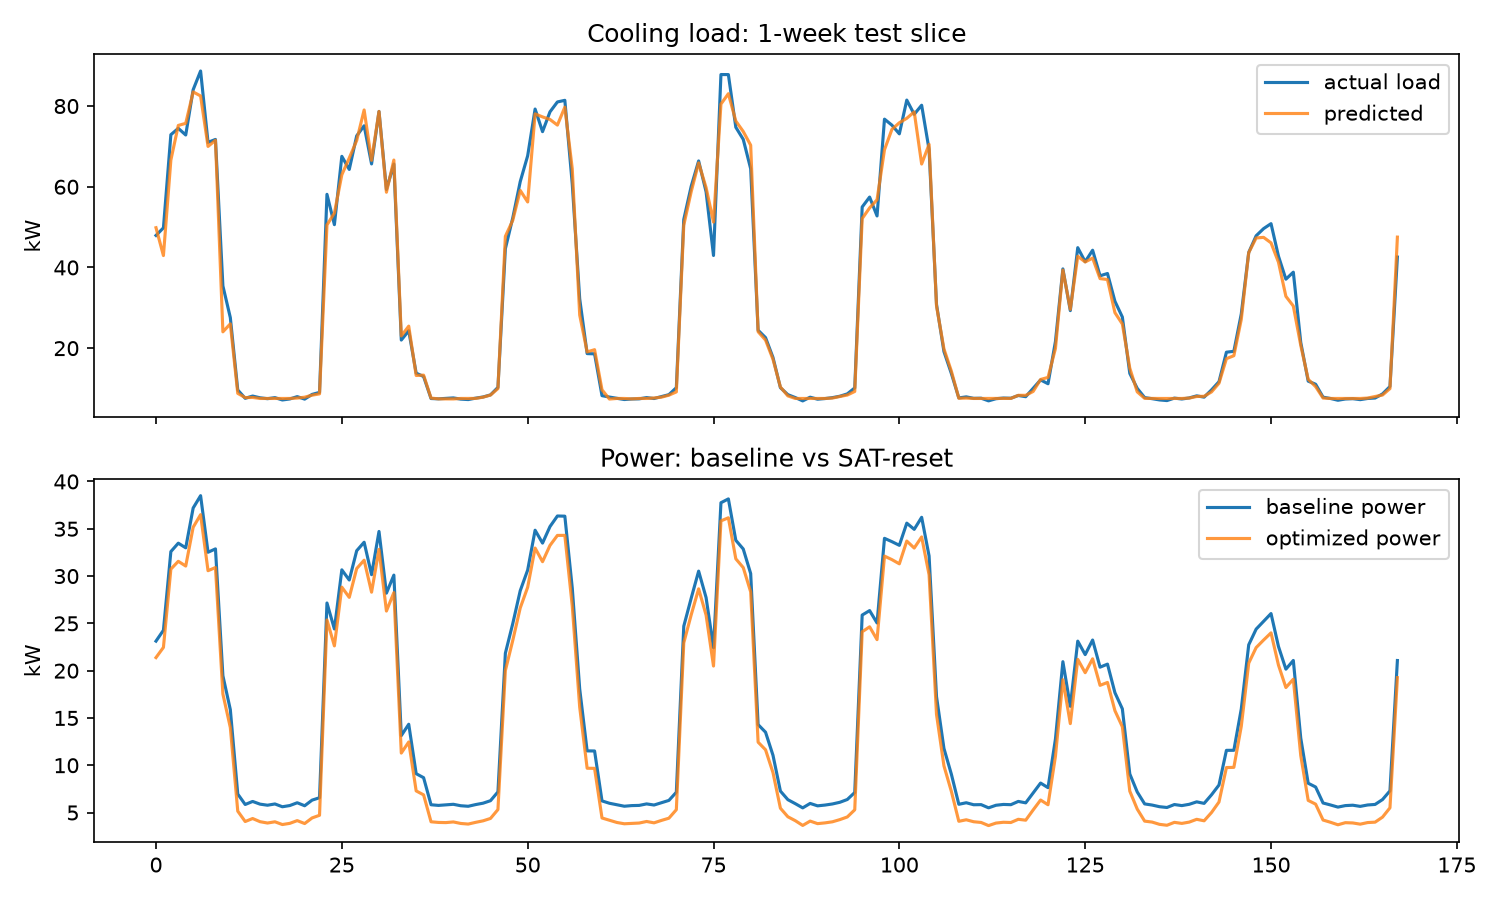
\includegraphics[width=3.4in]{demo.png}
\caption{One-week load forecast (top) and baseline vs.\ reset power (bottom).}
\label{fig:demo}
\end{figure}

\subsection{Simulation Sanity}
The 2R2C loop at 34$^\circ$C engages cooling after hour one with COP in [1.5, 5]. All tests green.

\section{Practical Implications}
Utilities can reuse the forecaster as customer baseline and feeder day-ahead input. Aggregators can bid reset/pre-cool kW with 2R2C-bounded rebound. Owners get sequencing plus reset with no new iron. Limits: synthetic data, proxy coefficients (relative savings claimed), no network/tariff/PMV constraints; OpenDSS feeder hosting with AMI data is next.

\section{Conclusion}
Physics-informed ML clears calibration grade and delivers 11--14\% energy and $\sim$10\% peak reduction per building with laptop tooling: a dispatchable GEB resource. Code, seeds, and CSV swap-in path are published for PES replication.

\section*{Acknowledgment}
Thanks to the NumPy, pandas, scikit-learn, and matplotlib communities.

\begin{thebibliography}{00}
\bibitem{ashrae2021} ASHRAE Handbook---Fundamentals, Ch.~1, 2021.
\bibitem{g14} ASHRAE Guideline 14-2014.
\bibitem{g36} ASHRAE Guideline 36-2024.
\bibitem{braun} J.~E.~Braun \textit{et al.}, Supervisory control of building HVAC, \textit{ASHRAE Trans.}
\bibitem{sklearn} F.~Pedregosa \textit{et al.}, Scikit-learn, \textit{JMLR}, vol.~12, 2011.
\bibitem{geb} S.~H.~Hong \textit{et al.}, Grid-interactive efficient buildings, \textit{IEEE Electrific. Mag.}
\bibitem{mpc} Y.~Ma \textit{et al.}, MPC for buildings survey, \textit{Appl.\ Energy}.
\end{thebibliography}

\end{document}
